\documentclass[11pt]{article}
\usepackage[margin=0.88in]{geometry}
\usepackage[T1]{fontenc}
\usepackage[utf8]{inputenc}
\usepackage{lmodern,microtype}
\usepackage{amsmath,amssymb,amsthm,mathtools,bm}
\usepackage[dvipsnames]{xcolor}
\usepackage{tikz}
\usetikzlibrary{arrows.meta,positioning,calc,fit,backgrounds,shapes.multipart,matrix}
\usepackage{hyperref}
\usepackage{enumitem}
\usepackage{float}
\usepackage{array}
\usepackage{booktabs}
\usepackage{longtable}
\hypersetup{colorlinks=true,linkcolor=MidnightBlue,urlcolor=MidnightBlue,citecolor=MidnightBlue,pdftitle={Formalized strategy diagram for Type-1, N=3 Landau-Zener},pdfauthor={OpenAI}}

\newcommand{\C}{\mathbb C}
\newcommand{\PP}{\mathbb P}
\newcommand{\ii}{\mathrm{i}}
\newcommand{\dd}{\mathrm{d}}
\newcommand{\Disc}{\operatorname{Disc}}
\newcommand{\diag}{\operatorname{diag}}
\newcommand{\CY}{\Sigma_Y}
\newcommand{\CR}{\Sigma_R}
\newcommand{\Chat}{\widehat{\mathcal C}}
\newcommand{\Cu}{\mathcal C}
\newcommand{\Eu}{\mathcal E}
\newcommand{\Hx}{\mathsf H_x}
\newcommand{\Yop}{\mathsf Y}
\newcommand{\Rop}{\mathsf R}
\newcommand{\CRam}{\mathfrak C_R}
\newcommand{\Selcand}{\mathrm{Sel}^{\mathrm{cand}}_{\theta}(H)}
\newcommand{\Selact}{\mathrm{Sel}^{\mathrm{act}}_{\theta}(H)}
\newcommand{\Turns}{\mathrm{Turn}(H)}
\newcommand{\Graph}{\mathfrak G_{H,\theta}}
\newcommand{\Tfun}{\mathcal T_{H,\theta}}
\newcommand{\PathGpd}{\Pi_1(\Graph)}
\newcommand{\Ord}{\mathrm{Ord}_{\theta}(H)}

\definecolor{TitleBlue}{HTML}{173753}
\definecolor{AccentBlue}{HTML}{2F5D7E}
\definecolor{SoftBlue}{HTML}{EEF4FA}
\definecolor{SoftGold}{HTML}{FAF6EE}
\definecolor{SoftGreen}{HTML}{EDF7F0}
\definecolor{LineBlue}{HTML}{B5CBD8}
\definecolor{MutedText}{HTML}{4E5A66}
\definecolor{OpenRed}{HTML}{B85450}
\definecolor{SoftGray}{HTML}{F5F7FA}

\newtheorem{definition}{Definition}[section]
\newtheorem{proposition}[definition]{Proposition}
\newtheorem{remark}[definition]{Remark}

\setlength{\parindent}{0pt}
\setlength{\parskip}{0.48em}
\setlist[itemize]{leftmargin=1.3em,itemsep=0.15em,topsep=0.2em}
\setlist[enumerate]{leftmargin=1.5em,itemsep=0.18em,topsep=0.2em}
\pagestyle{empty}
\renewcommand{\arraystretch}{1.14}
\newcolumntype{P}[1]{>{\raggedright\arraybackslash}p{#1}}

\begin{document}

\begin{center}
{\Large\bfseries\color{TitleBlue}Formal objects, morphisms, and glossary for the Type-1, $N=3$ Landau--Zener reduction\par}
\vspace{0.35em}
{\large\color{AccentBlue}shared geometry, selector data, and the continuation functor\par}
\end{center}

This note formalizes the two diagrams in the strategy document.  It does two things.
First, it replaces each box by a named mathematical object.  Second, it replaces each arrow by a named map, process, or partially defined morphism.  The resulting diagram is meant to be inspected by a mathematician who has not seen the project before: the base ODE sits at the left, the shared spectral geometry in the middle, and the unresolved exact-WKB data are concentrated in a single broken morphism on the right.

The note builds on the augmented adiabatic-basis ODE, the quotient-ring reduction, the commuting triple $(\Hx,\Yop,\Rop)$, and the common-cover / selector framework developed in the summary and primer.

\section{Foundational geometric objects inherited from the summary and primer}

We fix a Type-1, $N=3$ commuting family, a member $H$, a preferred incoming channel $x$, and a Borel direction $\theta$.  The family-invariant spectral data are the rational functions
\[
q_u(\lambda)=u\,p(\lambda)-n(\lambda),
\qquad
u(\lambda)=\frac{n(\lambda)}{p(\lambda)},
\qquad
E(\lambda)=\frac{m_H(\lambda)}{p(\lambda)}.
\]
The gauged adiabatic amplitudes satisfy
\[
f'(u)=\bigl[-S(u)+\ii D_H(u)\bigr]f(u),
\]
where $S$ is the transport connection of the moving adiabatic frame and $D_H$ is diagonal in the adiabatic basis.

For $N=3$, the squared pairwise gaps live on the cubic phase curve
\[
\chi_Y(u,y)=y^3-2A(u)y^2+A(u)^2y-D(u)=0,
\]
and the transport coordinate is
\[
r(\lambda)=\frac{W_4(\lambda)}{L_H(\lambda)^4}.
\]
The common phase--transport cover and its spinor lift are
\[
\Cu=\CY\times_{\PP^1_u}\CR,
\qquad
\Chat=\{(u,y,r,\rho)\in \Cu\times\C:\rho^2=\kappa_S/r\},
\]
with global one-forms
\[
\omega=\sqrt{y}\,\dd u,
\qquad
\eta=S\,\dd u=\frac{\rho}{y}\,\dd u.
\]
The commuting triple is
\[
(\Hx,\Yop,\Rop),
\qquad
\Yop=M_{Q_4L_H^2/p^2},
\qquad
\Rop=M_{W_4/L_H^4}.
\]
Away from the transport discriminant
\[
\CRam=\{u\in\PP^1_u:\Disc_r\chi_R(u,r)=0\},
\]
the spectral projectors of $\Rop$ define the canonical splitting
\[
\Eu_u=\mathcal L_1(u)\oplus \mathcal L_2(u)\oplus \mathcal L_3(u).
\]
This is the precise sense in which gluing is already solved on the regular set.

\section{Formal reduction objects}

We now package the strategy into named objects.

\begin{definition}[Base ODE object]
\label{def:base-object}
The \emph{base ODE object} is
\[
\mathbf B_{H,x}:=(U,\mathcal F_{H,x},\nabla^{\mathrm{ad}}_{H,x}),
\qquad
\mathcal F_{H,x}:=U\times\C^3,
\qquad
\nabla^{\mathrm{ad}}_{H,x}:=\partial_u+S(u)-\ii D_H(u),
\]
so that $\nabla^{\mathrm{ad}}_{H,x}f=0$ is the gauged adiabatic-basis equation.
\end{definition}

\begin{definition}[Reduced algebraic object]
\label{def:reduced-object}
The \emph{reduced algebraic object} is
\[
\mathbf Q_{H,x}:=(U,\Eu,\nabla^{\mathrm{red}}_{H,x};q_u,s_u),
\qquad
\Eu_u:=\C[\lambda]/(q_u(\lambda)),
\qquad
\nabla^{\mathrm{red}}_{H,x}:=\partial_u-\ii\Hx,
\]
where $s_u$ is the inverse of $p$ in $\Eu_u$ and $\Hx=M_{h_x}$ with
\[
h_x(\lambda;u)=\operatorname{red}_{q_u}\bigl((m_H(\lambda)-E_x(u)p(\lambda))s_u(\lambda)\bigr).
\]
\end{definition}

\begin{definition}[Commuting algebra object]
\label{def:alg-object}
The \emph{commuting algebra object} is
\[
\mathbf A_H:=(\Eu,\Hx,\Yop,\Rop),
\]
where $\Yop$ and $\Rop$ are the multiplication operators with symbols
\[
\mathfrak y(\lambda)=\frac{Q_4(\lambda)L_H(\lambda)^2}{p(\lambda)^2},
\qquad
\mathfrak r(\lambda)=\frac{W_4(\lambda)}{L_H(\lambda)^4}.
\]
\end{definition}

\begin{definition}[Spectral geometry object]
\label{def:geom-object}
The \emph{spectral geometry object} is
\[
\mathbf G_H:=(\CY,\CR,\Cu,\Chat;\omega,\eta),
\]
where
\[
\CY=\{(u,y):\chi_Y(u,y)=0\},
\qquad
\CR=\{(u,r):\chi_R(u,r)=0\},
\qquad
\Cu=\CY\times_{\PP^1_u}\CR,
\qquad
\Chat=\{\rho^2=\kappa_S/r\},
\]
and $\omega,\eta$ are the global phase and transport one-forms on $\Chat$.
\end{definition}

\begin{definition}[Ramification object]
\label{def:ram-object}
The \emph{ramification object} is
\[
\mathbf R_H:=(B_R,\CRam,\pi_R),
\]
where $\pi_R:\CR\to \PP^1_u$ is the projection, $B_R:=\mathrm{Ram}(\pi_R)$ is its ramification divisor, and $\CRam:=\pi_R(B_R)$ is the transport discriminant locus.
\end{definition}

\begin{definition}[Candidate selector object]
\label{def:candidate-object}
The \emph{candidate selector object} is
\[
\mathbf S^{\mathrm{cand}}_{H,\theta}:=(\Selcand,\mathcal S_{+-}),
\]
where
\[
\Selcand:=\Bigl\{u_*\in\CRam:\im\bigl(e^{-\ii\theta}\mathcal S_{+-}(u_*;H)\bigr)=0\Bigr\},
\qquad
\mathcal S_{+-}(u):=\int_{\gamma_{+-}(u)}\omega.
\]
\end{definition}

\begin{definition}[Local activation--multiplier object]
\label{def:local-jump-object}
The \emph{local activation--multiplier object} is
\[
\mathbf J_{H,\theta}:=(\Selact,\{J_s(H)\}_{s\in\Selact}),
\]
where $\Selact\subseteq \Selcand$ is the actual selector subset and $J_s(H)\in GL_3(\C)$ is the local jump matrix attached to $s$.
\end{definition}

\begin{remark}
Object~\ref{def:local-jump-object} is the only object in the chain that is not presently known by a closed intrinsic construction.  Determining it is the content of the unresolved local exact-WKB problem.
\end{remark}

\begin{definition}[Decorated continuation graph]
\label{def:graph-object}
The \emph{decorated continuation graph} is
\[
\mathbf G^{\mathrm{dec}}_{H,\theta}:=(\Graph,V,E,\ell),
\]
where
\[
V=\Ord\cup\Selact\cup V_\infty,
\]
with $\Ord$ the ordinary turning-point set and $V_\infty$ the chosen asymptotic sector vertices.  The edges are the Stokes and transport sectors between these vertices, and the label function $\ell$ assigns propagation data to edges and local jump data to vertices.
\end{definition}

\begin{definition}[Path groupoid and continuation functor]
\label{def:groupoid-functor-objects}
The \emph{path groupoid object} is
\[
\mathbf P_{H,\theta}:=\PathGpd=\Pi_1(\Graph),
\]
and the \emph{continuation functor object} is
\[
\mathbf T_{H,\theta}:=(\PathGpd,\Tfun),
\qquad
\Tfun:\PathGpd\to GL_3(\C).
\]
\end{definition}

\begin{definition}[Output object]
\label{def:output-object}
The \emph{output object} is
\[
\mathbf O_{H,\theta}:=(f(+\infty),P),
\qquad
P_{x\to j}=|f_j(+\infty)|^2.
\]
\end{definition}

\section{Named morphisms and processes}

The arrows in the category-style diagram are the following constructions.

\begin{definition}[Spectral reduction and interpolation]
\label{def:q-map}
The map
\[
\mathfrak q_{H,x}:\mathbf B_{H,x}\longrightarrow \mathbf Q_{H,x}
\]
is defined by passing from the adiabatic coefficients $f_i$ to the reduced sheet carriers $R_i=f_i/\Gamma_i$, and then to the unique interpolation class $[R]\in\Eu_u$ with values $R(\lambda_i(u);u)=R_i(u)$.
\end{definition}

\begin{definition}[Adjoining the commuting multipliers]
\label{def:a-map}
The map
\[
\mathfrak a_H:\mathbf Q_{H,x}\longrightarrow \mathbf A_H
\]
keeps the same quotient-ring bundle and connection and adjoins the multiplication operators $\Yop$ and $\Rop$.
\end{definition}

\begin{definition}[Spectral-curve construction]
\label{def:s-map}
The map
\[
\mathfrak s_H:\mathbf A_H\longrightarrow \mathbf G_H
\]
assigns to the commuting algebra its spectral curves $\CY=\operatorname{Spec}(\Yop)$ and $\CR=\operatorname{Spec}(\Rop)$, their fiber product $\Cu$, the spinor lift $\Chat$, and the one-forms $\omega,\eta$.
\end{definition}

\begin{definition}[Ramification extraction]
\label{def:b-map}
The map
\[
\mathfrak b_H:\mathbf G_H\longrightarrow \mathbf R_H
\]
extracts the transport ramification divisor of the projection $\pi_R:\CR\to\PP^1_u$ and its image in the base.
\end{definition}

\begin{definition}[Phase-resonance sieve]
\label{def:c-map}
The map
\[
\mathfrak c_{H,\theta}:\mathbf G_H\longrightarrow \mathbf S^{\mathrm{cand}}_{H,\theta}
\]
is the function
\[
\mathbf G_H\longmapsto \left(\left\{u_*\in\CRam:\im\bigl(e^{-\ii\theta}\mathcal S_{+-}(u_*;H)\bigr)=0\right\},\ \mathcal S_{+-}\right).
\]
It is the formal version of ``transport ramification plus phase resonance.''
\end{definition}

\begin{definition}[Local activation--multiplier morphism]
\label{def:j-map}
The partially defined morphism
\[
\mathfrak j_{H,\theta}:\mathbf S^{\mathrm{cand}}_{H,\theta}\dashrightarrow \mathbf J_{H,\theta}
\]
assigns to the candidate selector object the actual active subset and its local jump matrices.
\end{definition}

\begin{remark}
The broken arrow notation in the diagram is intentional: $\mathfrak j_{H,\theta}$ is the unresolved local analytic input.  Every other arrow in the reduction is already formalized.
\end{remark}

\begin{definition}[Graph decoration]
\label{def:d-map}
The map
\[
\mathfrak d_{H,\theta}: (\mathbf G_H,\mathbf J_{H,\theta})\longrightarrow \mathbf G^{\mathrm{dec}}_{H,\theta}
\]
builds the decorated continuation graph by adjoining the ordinary turning set, the active selector set, and the corresponding edge/vertex labels.
\end{definition}

\begin{definition}[Fundamental-groupoid construction]
\label{def:p-map}
The map
\[
\mathfrak p_{H,\theta}:\mathbf G^{\mathrm{dec}}_{H,\theta}\longrightarrow \mathbf P_{H,\theta}
\]
assigns to the decorated graph its path groupoid.
\end{definition}

\begin{definition}[Ordered-product continuation functor]
\label{def:t-map}
The map
\[
\mathfrak t_{H,\theta}:\mathbf P_{H,\theta}\longrightarrow \mathbf T_{H,\theta}
\]
assigns to each morphism class in $\PathGpd$ the corresponding ordered product of edge propagators and local jump matrices.  On generators,
\[
\Tfun(e)=D_e(H),
\qquad
\Tfun(s)=J_s(H),
\]
and on composites it is multiplicative.
\end{definition}

\begin{definition}[Evaluation]
\label{def:e-map}
For a chosen continuation word $\gamma\in \PathGpd$, the evaluation map
\[
\mathfrak e_{H,\theta,\gamma}:\mathbf T_{H,\theta}\longrightarrow \mathbf O_{H,\theta}
\]
is given by
\[
\mathfrak e_{H,\theta,\gamma}(\Tfun)=\bigl(\Tfun(\gamma)f(-\infty),\ |\Tfun(\gamma)f(-\infty)|^2\bigr).
\]
\end{definition}

\begin{proposition}[Reduction up to the unresolved local step]
\label{prop:reduction-up-to-step5}
Once the local activation--multiplier morphism $\mathfrak j_{H,\theta}$ is supplied, the long-time Landau--Zener amplitudes are determined functorially by the composition
\[
\mathbf B_{H,x}
\xrightarrow{\mathfrak q_{H,x}}
\mathbf Q_{H,x}
\xrightarrow{\mathfrak a_H}
\mathbf A_H
\xrightarrow{\mathfrak s_H}
\mathbf G_H
\xrightarrow{\mathfrak c_{H,\theta}}
\mathbf S^{\mathrm{cand}}_{H,\theta}
\xrightarrow{\mathfrak j_{H,\theta}}
\mathbf J_{H,\theta}
\xrightarrow{\mathfrak d_{H,\theta}}
\mathbf G^{\mathrm{dec}}_{H,\theta}
\xrightarrow{\mathfrak p_{H,\theta}}
\mathbf P_{H,\theta}
\xrightarrow{\mathfrak t_{H,\theta}}
\mathbf T_{H,\theta}
\xrightarrow{\mathfrak e_{H,\theta,\gamma}}
\mathbf O_{H,\theta}.
\]
\end{proposition}

\begin{figure}[H]
\centering
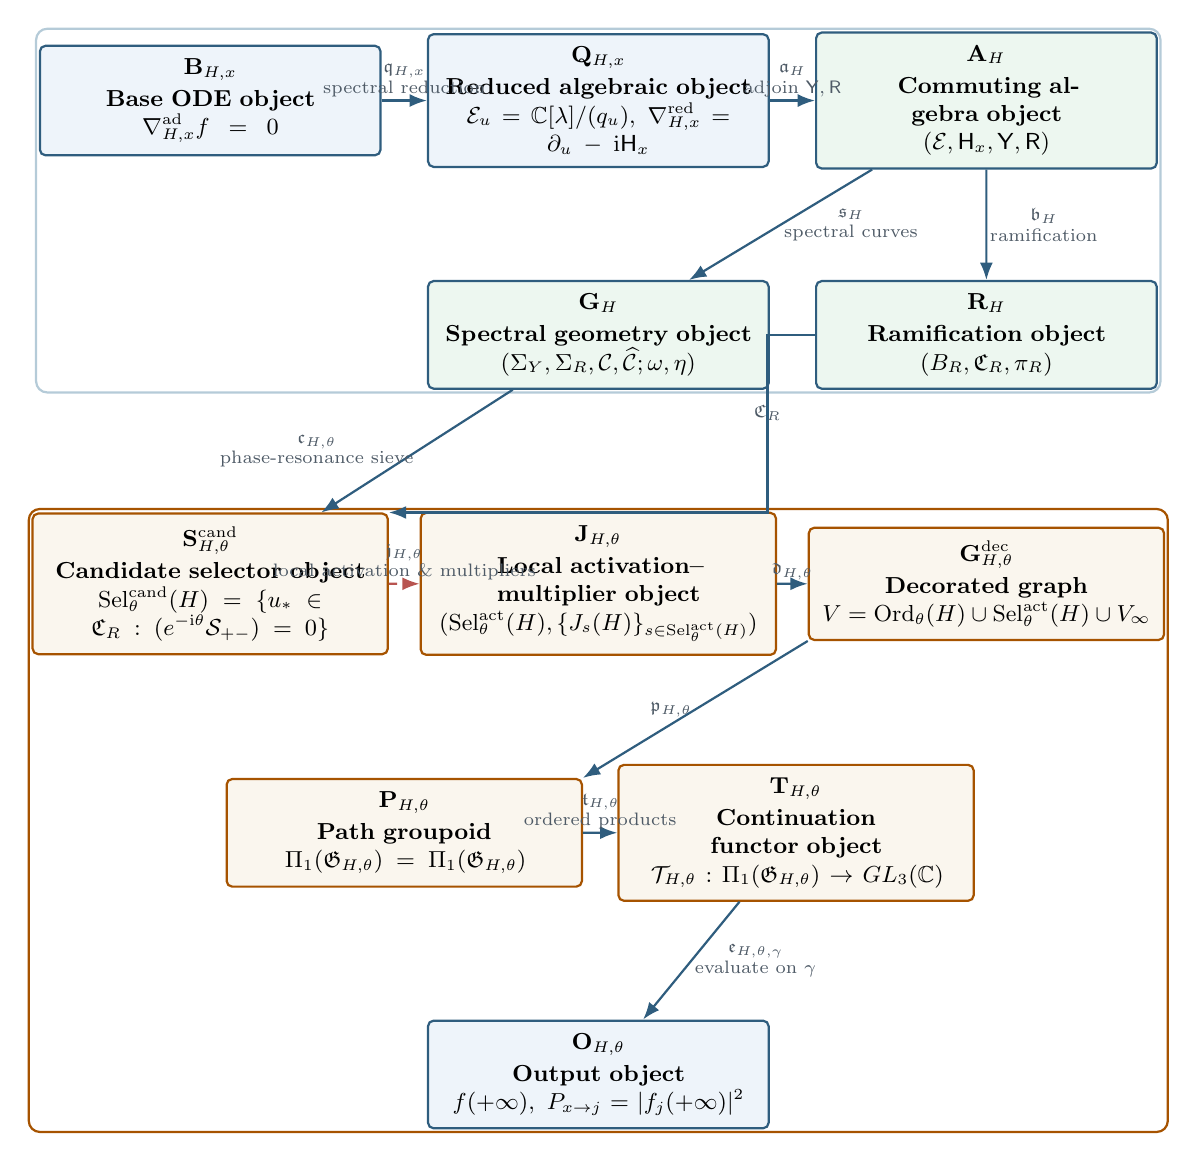
\begin{tikzpicture}[
  x=1cm,y=1cm, scale=0.93, transform shape,
  >={Latex[length=2.2mm]},
  box/.style={draw=AccentBlue, rounded corners=2pt, thick, fill=SoftBlue, align=center, inner sep=5pt, text width=4.3cm, font=\small},
  solved/.style={draw=AccentBlue, rounded corners=2pt, thick, fill=SoftGreen, align=center, inner sep=5pt, text width=4.3cm, font=\small},
  openbox/.style={draw=orange!65!black, rounded corners=2pt, thick, fill=SoftGold, align=center, inner sep=5pt, text width=4.5cm, font=\small},
  arrow/.style={->, thick, draw=AccentBlue},
  openarrow/.style={->, thick, dashed, draw=OpenRed},
  label/.style={font=\scriptsize, text=MutedText, inner sep=1pt, align=center}
]

\node[box] (B) at (0,0) {$\mathbf B_{H,x}$\\[0.15em]\textbf{Base ODE object}\\$\nabla^{\mathrm{ad}}_{H,x}f=0$};
\node[box] (Q) at (5.3,0) {$\mathbf Q_{H,x}$\\[0.15em]\textbf{Reduced algebraic object}\\$\Eu_u=\C[\lambda]/(q_u),\ \nabla^{\mathrm{red}}_{H,x}=\partial_u-\ii\Hx$};
\node[solved] (A) at (10.6,0) {$\mathbf A_H$\\[0.15em]\textbf{Commuting algebra object}\\$(\Eu,\Hx,\Yop,\Rop)$};

\node[solved] (G) at (5.3,-3.2) {$\mathbf G_H$\\[0.15em]\textbf{Spectral geometry object}\\$(\CY,\CR,\Cu,\Chat;\omega,\eta)$};
\node[solved] (R) at (10.6,-3.2) {$\mathbf R_H$\\[0.15em]\textbf{Ramification object}\\$(B_R,\CRam,\pi_R)$};
\node[openbox] (S) at (0,-6.6) {$\mathbf S^{\mathrm{cand}}_{H,\theta}$\\[0.15em]\textbf{Candidate selector object}\\$\Selcand=\{u_*\in\CRam:\im(e^{-\ii\theta}\mathcal S_{+-})=0\}$};
\node[openbox] (J) at (5.3,-6.6) {$\mathbf J_{H,\theta}$\\[0.15em]\textbf{Local activation--multiplier object}\\$(\Selact,\{J_s(H)\}_{s\in\Selact})$};
\node[openbox] (GD) at (10.6,-6.6) {$\mathbf G^{\mathrm{dec}}_{H,\theta}$\\[0.15em]\textbf{Decorated graph}\\$V=\Ord\cup\Selact\cup V_\infty$};

\node[openbox] (P) at (2.65,-10.0) {$\mathbf P_{H,\theta}$\\[0.15em]\textbf{Path groupoid}\\$\PathGpd=\Pi_1(\Graph)$};
\node[openbox] (T) at (8.0,-10.0) {$\mathbf T_{H,\theta}$\\[0.15em]\textbf{Continuation functor object}\\$\Tfun:\PathGpd\to GL_3(\C)$};
\node[box] (O) at (5.3,-13.3) {$\mathbf O_{H,\theta}$\\[0.15em]\textbf{Output object}\\$f(+\infty),\ P_{x\to j}=|f_j(+\infty)|^2$};

\draw[arrow] (B) -- node[label,above] {$\mathfrak q_{H,x}$\\spectral reduction} (Q);
\draw[arrow] (Q) -- node[label,above] {$\mathfrak a_H$\\adjoin $\Yop,\Rop$} (A);
\draw[arrow] (A) -- node[label,right] {$\mathfrak s_H$\\spectral curves} (G);
\draw[arrow] (A) -- node[label,right] {$\mathfrak b_H$\\ramification} (R);
\draw[arrow] (G) -- node[label,left] {$\mathfrak c_{H,\theta}$\\phase-resonance sieve} (S);
\draw[arrow] (R.west) -- ++(-0.65,0) |- node[label,pos=0.25,above] {$\CRam$} (S.north east);
\draw[openarrow] (S) -- node[label,above] {$\mathfrak j_{H,\theta}$\\local activation \& multipliers} (J);
\draw[arrow] (J) -- node[label,above] {$\mathfrak d_{H,\theta}$} (GD);
\draw[arrow] (GD.south west) -- node[label,left] {$\mathfrak p_{H,\theta}$} (P.north east);
\draw[arrow] (P) -- node[label,above] {$\mathfrak t_{H,\theta}$\\ordered products} (T);
\draw[arrow] (T) -- node[label,right] {$\mathfrak e_{H,\theta,\gamma}$\\evaluate on $\gamma$} (O);

\begin{scope}[on background layer]
  \node[draw=LineBlue, rounded corners=4pt, thick, inner sep=11pt, fit=(B)(Q)(A)(G)(R), label={[label]above:shared geometry and already formalized reduction}] {};
  \node[draw=orange!65!black, rounded corners=4pt, thick, inner sep=11pt, fit=(S)(J)(GD)(P)(T)(O), label={[label]above:remaining exact-WKB stage}] {};
\end{scope}

\end{tikzpicture}
\caption{\textbf{Formal strategy diagram with named objects and arrows.}  Every box is now a formally defined object.  Every arrow is a named map or process from Section~3.  The only broken arrow is $\mathfrak j_{H,\theta}$: the local activation--multiplier morphism that turns candidate selector points into active selector points equipped with jump matrices.}
\label{fig:strategy}
\end{figure}

\begin{figure}[H]
\centering
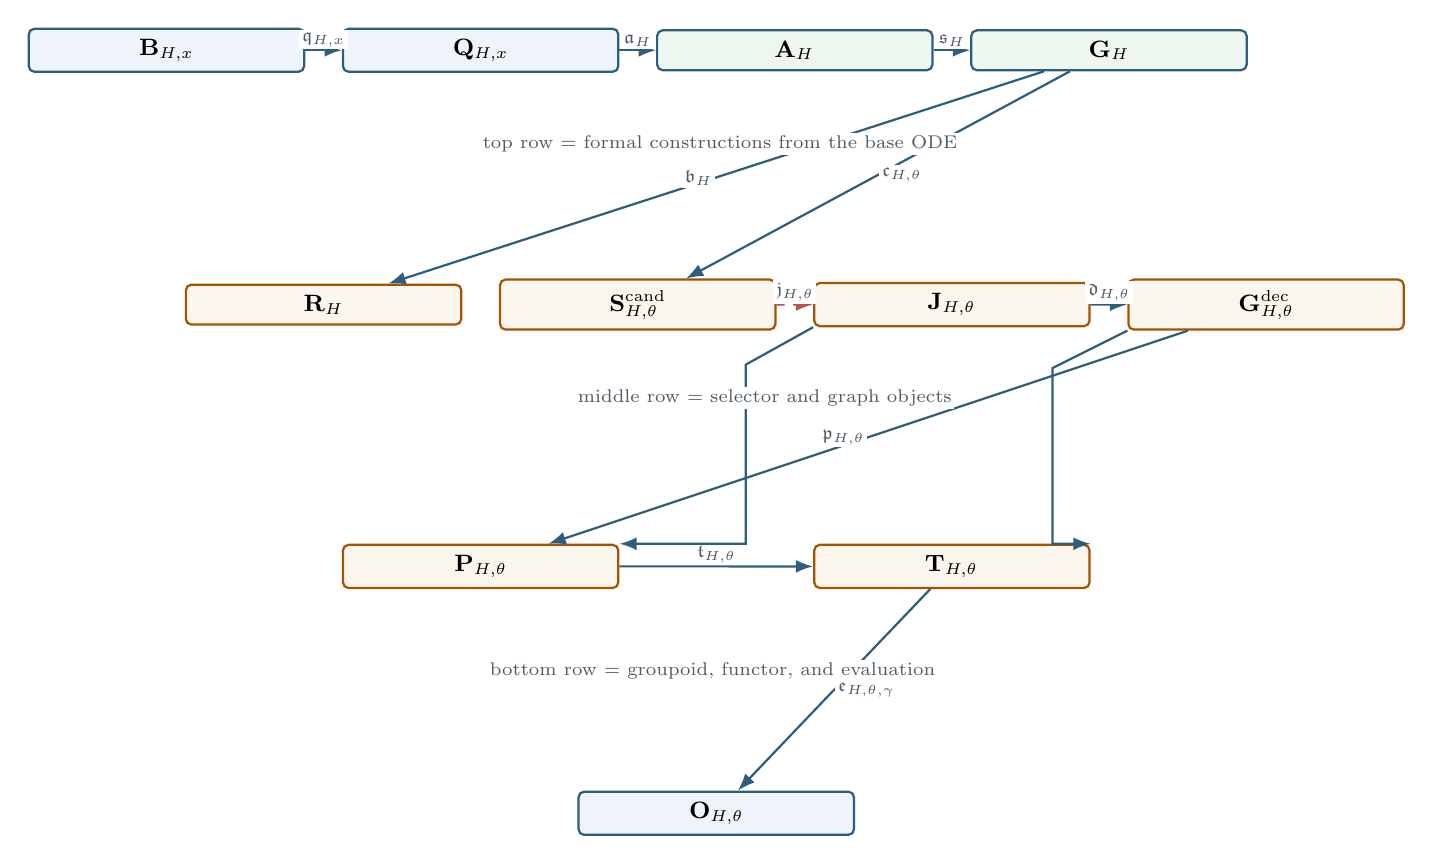
\begin{tikzpicture}[
  x=1cm,y=1cm, scale=0.95, transform shape,
  >={Latex[length=2.2mm]},
  obj/.style={draw=AccentBlue, rounded corners=2pt, thick, fill=SoftBlue, align=center, inner sep=4pt, text width=3.4cm, font=\small},
  geom/.style={draw=AccentBlue, rounded corners=2pt, thick, fill=SoftGreen, align=center, inner sep=4pt, text width=3.4cm, font=\small},
  openobj/.style={draw=orange!65!black, rounded corners=2pt, thick, fill=SoftGold, align=center, inner sep=4pt, text width=3.4cm, font=\small},
  morph/.style={->, thick, draw=AccentBlue},
  openmorph/.style={->, thick, dashed, draw=OpenRed},
  mlabel/.style={font=\scriptsize, text=MutedText, fill=white, inner sep=1pt, align=center}
]

\node[obj] (B) at (0,0) {$\mathbf B_{H,x}$};
\node[obj] (Q) at (4.2,0) {$\mathbf Q_{H,x}$};
\node[geom] (A) at (8.4,0) {$\mathbf A_H$};
\node[geom] (G) at (12.6,0) {$\mathbf G_H$};

\node[openobj] (R) at (2.1,-3.4) {$\mathbf R_H$};
\node[openobj] (S) at (6.3,-3.4) {$\mathbf S^{\mathrm{cand}}_{H,\theta}$};
\node[openobj] (J) at (10.5,-3.4) {$\mathbf J_{H,\theta}$};
\node[openobj] (GD) at (14.7,-3.4) {$\mathbf G^{\mathrm{dec}}_{H,\theta}$};

\node[openobj] (P) at (4.2,-6.9) {$\mathbf P_{H,\theta}$};
\node[openobj] (T) at (10.5,-6.9) {$\mathbf T_{H,\theta}$};
\node[obj] (O) at (7.35,-10.2) {$\mathbf O_{H,\theta}$};

\draw[morph] (B) -- node[mlabel,above] {$\mathfrak q_{H,x}$} (Q);
\draw[morph] (Q) -- node[mlabel,above] {$\mathfrak a_H$} (A);
\draw[morph] (A) -- node[mlabel,above] {$\mathfrak s_H$} (G);
\draw[morph] (G) -- node[mlabel,left] {$\mathfrak b_H$} (R);
\draw[morph] (G) -- node[mlabel,right] {$\mathfrak c_{H,\theta}$} (S);
\draw[openmorph] (S) -- node[mlabel,above] {$\mathfrak j_{H,\theta}$} (J);
\draw[morph] (J) -- node[mlabel,above] {$\mathfrak d_{H,\theta}$} (GD);
\draw[morph] (GD) -- node[mlabel,left] {$\mathfrak p_{H,\theta}$} (P);
\draw[morph] (P) -- node[mlabel,above] {$\mathfrak t_{H,\theta}$} (T);
\draw[morph] (T) -- node[mlabel,right] {$\mathfrak e_{H,\theta,\gamma}$} (O);

\draw[morph] (J.south west) -- ++(-0.9,-0.5) |- (P.north east);
\draw[morph] (GD.south west) -- ++(-1.0,-0.5) |- (T.north east);

\node[mlabel] at (7.4,-1.25) {top row = formal constructions from the base ODE};
\node[mlabel] at (8.0,-4.65) {middle row = selector and graph objects};
\node[mlabel] at (7.3,-8.3) {bottom row = groupoid, functor, and evaluation};

\end{tikzpicture}
\caption{\textbf{Category-style reduction diagram.}  The reduction is organized as a chain of named objects and named morphisms.  The only non-formalized morphism is the dashed map $\mathfrak j_{H,\theta}$, which must decide which candidate selector points are genuinely active and what local jump matrices they carry.}
\label{fig:category}
\end{figure}

\section{Glossary of foundational objects (from the summary and primer, augmented)}

\small
\begin{longtable}{P{0.17\linewidth}P{0.27\linewidth}P{0.46\linewidth}}
\toprule
\textbf{Symbol} & \textbf{Definition} & \textbf{Role in the reduction}\\
\midrule
\endfirsthead
\toprule
\textbf{Symbol} & \textbf{Definition} & \textbf{Role in the reduction}\\
\midrule
\endhead
$q_u(\lambda)$ & $u\,p(\lambda)-n(\lambda)$ & Spectral polynomial defining the quotient-ring fiber.\\
$\Eu_u$ & $\C[\lambda]/(q_u)$ & Rank-three fiber algebra that packages the three spectral sheets.\\
$[R]$ & Interpolation class in $\Eu_u$ with values $R(\lambda_i(u);u)$ at the roots of $q_u$ & Intrinsic reduced carrier.\\
$\Hx$ & Multiplication by $h_x=\operatorname{red}_{q_u}((m_H-E_xp)s_u)$ & Quotient-ring Hamiltonian for the reduced evolution.\\
$\Yop$ & Multiplication by $Q_4L_H^2/p^2$ & Operator whose spectrum gives $y=\Delta^2$.\\
$\Rop$ & Multiplication by $W_4/L_H^4$ & Operator whose spectrum gives the transport coordinate $r$.\\
$\CY$ & $\{(u,y):\chi_Y(u,y)=0\}$ & Global phase curve for squared gaps.\\
$\CR$ & $\{(u,r):\chi_R(u,r)=0\}$ & Global transport curve.\\
$\Cu$ & $\CY\times_{\PP^1_u}\CR$ & Common phase--transport cover.\\
$\Chat$ & $\{(u,y,r,\rho):\rho^2=\kappa_S/r\}$ & Spinor lift resolving the transport square root.\\
$\omega$ & $\sqrt{y}\,\dd u$ & Phase differential used in action comparison.\\
$\eta$ & $\rho\,\dd u/y$ & Transport differential on the spinor lift.\\
$B_R$ & $\mathrm{Ram}(\pi_R)$ for $\pi_R:\CR\to\PP^1_u$ & Transport-side branch locus upstairs.\\
$\CRam$ & $\pi_R(B_R)=\{u:\Disc_r\chi_R(u,r)=0\}$ & Transport discriminant locus downstairs.\\
$\mathcal S_{+-}$ & $\int_{\gamma_{+-}}\omega$ & Phase mismatch between the two locally colliding transport sheets.\\
$\Ord$ & Ordinary turning-point set, equivalently the zero set of the phase discriminant & Ordinary Stokes vertices.\\
\bottomrule
\end{longtable}
\normalsize

\section{Glossary of strategy objects (new in this note)}

\small
\begin{longtable}{P{0.18\linewidth}P{0.30\linewidth}P{0.42\linewidth}}
\toprule
\textbf{Object} & \textbf{Formal definition} & \textbf{Interpretation}\\
\midrule
\endfirsthead
\toprule
\textbf{Object} & \textbf{Formal definition} & \textbf{Interpretation}\\
\midrule
\endhead
$\mathbf B_{H,x}$ & Definition~\ref{def:base-object} & The original gauged adiabatic Landau--Zener problem as a connection on a trivial rank-three bundle.\\
$\mathbf Q_{H,x}$ & Definition~\ref{def:reduced-object} & The reduced quotient-ring formulation of the same dynamics.\\
$\mathbf A_H$ & Definition~\ref{def:alg-object} & The commuting algebra $(\Eu,\Hx,\Yop,\Rop)$ that simultaneously controls phase and transport.\\
$\mathbf G_H$ & Definition~\ref{def:geom-object} & The spectral geometry extracted from the commuting algebra.\\
$\mathbf R_H$ & Definition~\ref{def:ram-object} & The transport ramification data.\\
$\mathbf S^{\mathrm{cand}}_{H,\theta}$ & Definition~\ref{def:candidate-object} & Ramification points filtered by phase resonance in Borel direction $\theta$.\\
$\mathbf J_{H,\theta}$ & Definition~\ref{def:local-jump-object} & The active selector subset together with its local jump matrices.\\
$\mathbf G^{\mathrm{dec}}_{H,\theta}$ & Definition~\ref{def:graph-object} & The continuation graph carrying ordinary and selector vertices and edge labels.\\
$\mathbf P_{H,\theta}$ & Definition~\ref{def:groupoid-functor-objects} & The path groupoid of the decorated continuation graph.\\
$\mathbf T_{H,\theta}$ & Definition~\ref{def:groupoid-functor-objects} & The matrix-valued continuation functor.\\
$\mathbf O_{H,\theta}$ & Definition~\ref{def:output-object} & The long-time amplitudes and probabilities.\\
\bottomrule
\end{longtable}
\normalsize

\section{Glossary of named morphisms and their status}

\small
\begin{longtable}{P{0.15\linewidth}P{0.18\linewidth}P{0.18\linewidth}P{0.38\linewidth}}
\toprule
\textbf{Morph./process} & \textbf{Domain} & \textbf{Codomain} & \textbf{Meaning / status}\\
\midrule
\endfirsthead
\toprule
\textbf{Morph./process} & \textbf{Domain} & \textbf{Codomain} & \textbf{Meaning / status}\\
\midrule
\endhead
$\mathfrak q_{H,x}$ & $\mathbf B_{H,x}$ & $\mathbf Q_{H,x}$ & Spectral reduction and interpolation. Already formalized.\\
$\mathfrak a_H$ & $\mathbf Q_{H,x}$ & $\mathbf A_H$ & Adjoin the commuting multipliers $\Yop$ and $\Rop$. Already formalized.\\
$\mathfrak s_H$ & $\mathbf A_H$ & $\mathbf G_H$ & Spectral-curve / fiber-product construction. Already formalized.\\
$\mathfrak b_H$ & $\mathbf G_H$ & $\mathbf R_H$ & Extract transport ramification data. Already formalized.\\
$\mathfrak c_{H,\theta}$ & $\mathbf G_H$ & $\mathbf S^{\mathrm{cand}}_{H,\theta}$ & Phase-resonance sieve: transport ramification plus Stokes-real phase mismatch. Already formalized as a rule.\\
$\mathfrak j_{H,\theta}$ & $\mathbf S^{\mathrm{cand}}_{H,\theta}$ & $\mathbf J_{H,\theta}$ & Local activation and multiplier assignment. \textbf{Open}.\\
$\mathfrak d_{H,\theta}$ & $(\mathbf G_H,\mathbf J_{H,\theta})$ & $\mathbf G^{\mathrm{dec}}_{H,\theta}$ & Decorate the graph by ordinary/selector vertices and local labels. Formal once $\mathfrak j_{H,\theta}$ is known.\\
$\mathfrak p_{H,\theta}$ & $\mathbf G^{\mathrm{dec}}_{H,\theta}$ & $\mathbf P_{H,\theta}$ & Fundamental-groupoid construction. Standard.\\
$\mathfrak t_{H,\theta}$ & $\mathbf P_{H,\theta}$ & $\mathbf T_{H,\theta}$ & Ordered-product continuation functor. Formal once local jumps are known.\\
$\mathfrak e_{H,\theta,\gamma}$ & $\mathbf T_{H,\theta}$ & $\mathbf O_{H,\theta}$ & Evaluate the continuation functor on a chosen continuation word and incoming state. Standard.\\
\bottomrule
\end{longtable}
\normalsize

\section{A concise reduction principle}

\begin{proposition}[What is solved, and what is left]
The formal reduction of the Type-1, $N=3$ Landau--Zener problem is complete up to the single broken morphism $\mathfrak j_{H,\theta}$.  Equivalently:
\begin{itemize}
\item the passage from the base ODE to the commuting algebra is formalized;
\item the passage from the commuting algebra to the common cover, spinor lift, and transport ramification locus is formalized;
\item the candidate selector set is formalized by the phase-resonance sieve;
\item the only genuinely missing analytic datum is the map that turns candidate selector points into active selector points carrying local jump matrices.
\end{itemize}
Once $\mathfrak j_{H,\theta}$ is known, the continuation functor and therefore the long-time amplitudes are determined by functorial assembly.
\end{proposition}

\begin{remark}
This is the sharpest sense in which the problem is now ``solvable up to step 5.''  The geometry, the algebra, the ramification, and the candidate-selector sieve are already formalized.  The unresolved content is concentrated in a single local exact-WKB assignment.
\end{remark}

\end{document}
